%% GENERATED by scripts/make_figure1.py -- edit the generator, not this file.
\documentclass[border=6pt]{standalone}
\usepackage{tikz}
\usetikzlibrary{arrows.meta}
\usepackage{sansmath}
\renewcommand{\familydefault}{\sfdefault}
\sansmath
\definecolor{ink}{HTML}{1B2430}
\definecolor{inkdim}{HTML}{5D7185}
\definecolor{gridc}{HTML}{C9D3DE}
\definecolor{sph}{HTML}{D9DEE4}
\definecolor{sub}{HTML}{C8CED6}
\definecolor{shellc}{HTML}{EEF1F5}
\definecolor{uhi}{HTML}{1D3A7A}
\definecolor{ulo}{HTML}{F5DFA0}
\definecolor{spA}{HTML}{1D3A7A}
\definecolor{spB}{HTML}{A4C639}
\definecolor{spAB}{HTML}{2BB3A3}
\tikzset{
  gridl/.style={draw=gridc, line width=0.5pt},
  gridb/.style={draw=gridc!70!ink, line width=0.6pt},
  shell/.style={fill=shellc},
  op/.style={-{Stealth[length=7pt,width=5pt]}, line width=1.4pt, ink},
  mv/.style={-{Stealth[length=4pt,width=3.5pt]}, line width=0.9pt, ink},
  gen/.style={-{Stealth[length=5pt]}, line width=0.9pt, inkdim},
  lbl/.style={font=\small, ink},
  reads/.style={-{Stealth[length=5pt]}, line width=0.9pt, inkdim, dashed},
}
\newcommand{\num}[1]{\tikz[baseline=(n.base)]\node[draw=ink, circle, line width=0.6pt, inner sep=0.8pt, font=\scriptsize](n){#1};}
\begin{document}
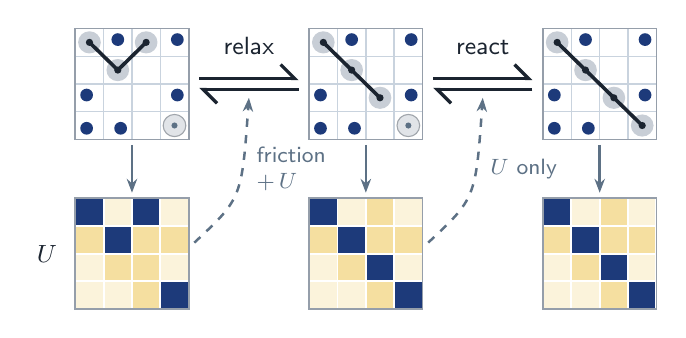
\begin{tikzpicture}[x=0.9cm, y=0.88cm]
\draw[gridl, shift={(4.150,-1.950)}] (0,0) grid[step=0.400] (1.600,1.600);
\draw[gridb] (4.150,-1.950) rectangle (5.750,-0.350);
\fill[sub] (4.350,-0.550) circle (0.160);
\fill[sub] (4.750,-0.950) circle (0.160);
\fill[sub] (5.150,-0.550) circle (0.160);
\fill[sub!55!white, draw=sub!80!black, line width=0.4pt] (5.550,-1.750) circle (0.160);
\fill[inkdim] (5.550,-1.750) circle (1.1pt);
\draw[ink, line width=1.3pt] (4.350,-0.550) -- (4.750,-0.950) -- (5.150,-0.550);
\fill[ink] (4.350,-0.550) circle (1.3pt);
\fill[ink] (4.750,-0.950) circle (1.3pt);
\fill[ink] (5.150,-0.550) circle (1.3pt);
\fill[spA] (4.310,-1.790) circle (2.3pt);
\fill[spA] (4.790,-1.790) circle (2.3pt);
\fill[spA] (4.310,-1.310) circle (2.3pt);
\fill[spA] (5.590,-1.310) circle (2.3pt);
\fill[spA] (5.590,-0.510) circle (2.3pt);
\fill[spA] (4.750,-0.510) circle (2.3pt);
\draw[gen] (4.950,-2.030) -- (4.950,-2.720);
\draw[gridl, shift={(7.450,-1.950)}] (0,0) grid[step=0.400] (1.600,1.600);
\draw[gridb] (7.450,-1.950) rectangle (9.050,-0.350);
\fill[sub] (7.650,-0.550) circle (0.160);
\fill[sub] (8.050,-0.950) circle (0.160);
\fill[sub] (8.450,-1.350) circle (0.160);
\fill[sub!55!white, draw=sub!80!black, line width=0.4pt] (8.850,-1.750) circle (0.160);
\fill[inkdim] (8.850,-1.750) circle (1.1pt);
\draw[ink, line width=1.3pt] (7.650,-0.550) -- (8.050,-0.950) -- (8.450,-1.350);
\fill[ink] (7.650,-0.550) circle (1.3pt);
\fill[ink] (8.050,-0.950) circle (1.3pt);
\fill[ink] (8.450,-1.350) circle (1.3pt);
\fill[spA] (7.610,-1.790) circle (2.3pt);
\fill[spA] (8.090,-1.790) circle (2.3pt);
\fill[spA] (7.610,-1.310) circle (2.3pt);
\fill[spA] (8.890,-1.310) circle (2.3pt);
\fill[spA] (8.890,-0.510) circle (2.3pt);
\fill[spA] (8.050,-0.510) circle (2.3pt);
\draw[gen] (8.250,-2.030) -- (8.250,-2.720);
\draw[gridl, shift={(10.750,-1.950)}] (0,0) grid[step=0.400] (1.600,1.600);
\draw[gridb] (10.750,-1.950) rectangle (12.350,-0.350);
\fill[sub] (10.950,-0.550) circle (0.160);
\fill[sub] (11.350,-0.950) circle (0.160);
\fill[sub] (11.750,-1.350) circle (0.160);
\fill[sub] (12.150,-1.750) circle (0.160);
\draw[ink, line width=1.3pt] (10.950,-0.550) -- (11.350,-0.950) -- (11.750,-1.350) -- (12.150,-1.750);
\fill[ink] (10.950,-0.550) circle (1.3pt);
\fill[ink] (11.350,-0.950) circle (1.3pt);
\fill[ink] (11.750,-1.350) circle (1.3pt);
\fill[ink] (12.150,-1.750) circle (1.3pt);
\fill[spA] (10.910,-1.790) circle (2.3pt);
\fill[spA] (11.390,-1.790) circle (2.3pt);
\fill[spA] (10.910,-1.310) circle (2.3pt);
\fill[spA] (12.190,-1.310) circle (2.3pt);
\fill[spA] (12.190,-0.510) circle (2.3pt);
\fill[spA] (11.350,-0.510) circle (2.3pt);
\draw[gen] (11.550,-2.030) -- (11.550,-2.720);
\draw[-{Straight Barb[left,length=5pt]}, line width=1.2pt, ink] (5.900,-1.070) -- (7.300,-1.070);
\draw[-{Straight Barb[left,length=5pt]}, line width=1.2pt, ink] (7.300,-1.230) -- (5.900,-1.230);
\node[lbl, above=7pt] at (6.600,-1.150) {relax};
\draw[reads] (5.830,-3.440) .. controls (6.500,-2.800) .. (6.600,-1.350);
\node[anchor=west, align=left, font=\footnotesize, inkdim, inner sep=0pt] at (6.700,-2.375) {friction\\$+\,U$};
\draw[-{Straight Barb[left,length=5pt]}, line width=1.2pt, ink] (9.200,-1.070) -- (10.600,-1.070);
\draw[-{Straight Barb[left,length=5pt]}, line width=1.2pt, ink] (10.600,-1.230) -- (9.200,-1.230);
\node[lbl, above=7pt] at (9.900,-1.150) {react};
\draw[reads] (9.130,-3.440) .. controls (9.800,-2.800) .. (9.900,-1.350);
\node[anchor=west, align=left, font=\footnotesize, inkdim, inner sep=0pt] at (10.000,-2.375) {$U$ only};
\node[lbl, anchor=east] at (4.030,-3.600) {$U$};
\fill[ulo!38!white] (4.150,-4.400) rectangle ++(0.400,0.400);
\fill[ulo!38!white] (4.550,-4.400) rectangle ++(0.400,0.400);
\fill[ulo!100!white] (4.950,-4.400) rectangle ++(0.400,0.400);
\fill[uhi!100!white] (5.350,-4.400) rectangle ++(0.400,0.400);
\fill[ulo!38!white] (4.150,-4.000) rectangle ++(0.400,0.400);
\fill[ulo!100!white] (4.550,-4.000) rectangle ++(0.400,0.400);
\fill[ulo!100!white] (4.950,-4.000) rectangle ++(0.400,0.400);
\fill[ulo!38!white] (5.350,-4.000) rectangle ++(0.400,0.400);
\fill[ulo!100!white] (4.150,-3.600) rectangle ++(0.400,0.400);
\fill[uhi!100!white] (4.550,-3.600) rectangle ++(0.400,0.400);
\fill[ulo!100!white] (4.950,-3.600) rectangle ++(0.400,0.400);
\fill[ulo!100!white] (5.350,-3.600) rectangle ++(0.400,0.400);
\fill[uhi!100!white] (4.150,-3.200) rectangle ++(0.400,0.400);
\fill[ulo!38!white] (4.550,-3.200) rectangle ++(0.400,0.400);
\fill[uhi!100!white] (4.950,-3.200) rectangle ++(0.400,0.400);
\fill[ulo!38!white] (5.350,-3.200) rectangle ++(0.400,0.400);
\draw[white, line width=0.7pt, shift={(4.150,-4.400)}] (0,0) grid[step=0.400] (1.600,1.600);
\draw[gridb] (4.150,-4.400) rectangle (5.750,-2.800);
\fill[ulo!38!white] (7.450,-4.400) rectangle ++(0.400,0.400);
\fill[ulo!38!white] (7.850,-4.400) rectangle ++(0.400,0.400);
\fill[ulo!100!white] (8.250,-4.400) rectangle ++(0.400,0.400);
\fill[uhi!100!white] (8.650,-4.400) rectangle ++(0.400,0.400);
\fill[ulo!38!white] (7.450,-4.000) rectangle ++(0.400,0.400);
\fill[ulo!100!white] (7.850,-4.000) rectangle ++(0.400,0.400);
\fill[uhi!100!white] (8.250,-4.000) rectangle ++(0.400,0.400);
\fill[ulo!38!white] (8.650,-4.000) rectangle ++(0.400,0.400);
\fill[ulo!100!white] (7.450,-3.600) rectangle ++(0.400,0.400);
\fill[uhi!100!white] (7.850,-3.600) rectangle ++(0.400,0.400);
\fill[ulo!100!white] (8.250,-3.600) rectangle ++(0.400,0.400);
\fill[ulo!100!white] (8.650,-3.600) rectangle ++(0.400,0.400);
\fill[uhi!100!white] (7.450,-3.200) rectangle ++(0.400,0.400);
\fill[ulo!38!white] (7.850,-3.200) rectangle ++(0.400,0.400);
\fill[ulo!100!white] (8.250,-3.200) rectangle ++(0.400,0.400);
\fill[ulo!38!white] (8.650,-3.200) rectangle ++(0.400,0.400);
\draw[white, line width=0.7pt, shift={(7.450,-4.400)}] (0,0) grid[step=0.400] (1.600,1.600);
\draw[gridb] (7.450,-4.400) rectangle (9.050,-2.800);
\fill[ulo!38!white] (10.750,-4.400) rectangle ++(0.400,0.400);
\fill[ulo!38!white] (11.150,-4.400) rectangle ++(0.400,0.400);
\fill[ulo!100!white] (11.550,-4.400) rectangle ++(0.400,0.400);
\fill[uhi!100!white] (11.950,-4.400) rectangle ++(0.400,0.400);
\fill[ulo!38!white] (10.750,-4.000) rectangle ++(0.400,0.400);
\fill[ulo!100!white] (11.150,-4.000) rectangle ++(0.400,0.400);
\fill[uhi!100!white] (11.550,-4.000) rectangle ++(0.400,0.400);
\fill[ulo!38!white] (11.950,-4.000) rectangle ++(0.400,0.400);
\fill[ulo!100!white] (10.750,-3.600) rectangle ++(0.400,0.400);
\fill[uhi!100!white] (11.150,-3.600) rectangle ++(0.400,0.400);
\fill[ulo!100!white] (11.550,-3.600) rectangle ++(0.400,0.400);
\fill[ulo!100!white] (11.950,-3.600) rectangle ++(0.400,0.400);
\fill[uhi!100!white] (10.750,-3.200) rectangle ++(0.400,0.400);
\fill[ulo!38!white] (11.150,-3.200) rectangle ++(0.400,0.400);
\fill[ulo!100!white] (11.550,-3.200) rectangle ++(0.400,0.400);
\fill[ulo!38!white] (11.950,-3.200) rectangle ++(0.400,0.400);
\draw[white, line width=0.7pt, shift={(10.750,-4.400)}] (0,0) grid[step=0.400] (1.600,1.600);
\draw[gridb] (10.750,-4.400) rectangle (12.350,-2.800);
\end{tikzpicture}
\end{document}
